\documentclass[11pt]{report}

% this one apparently fixes the < and > chars
\usepackage[T1]{fontenc}
\usepackage{subfigure}
\usepackage{times}
\usepackage{tabularx}

% why did we need this?
%\usepackage{verbatim}
% make all captions small and slanted
\usepackage[small,sl]{caption}
\usepackage{fullpage}
%\usepackage{epsf}
\usepackage{epsfig}
\usepackage{graphicx}
% add nifty DRAFT watermark thingy in PS
%\usepackage{draftcopy}

% A nice environment for displaying command line args (AH)
\newenvironment{xarg}[1]{\noindent{\tt #1}\\\hspace*{2em}\begin{minipage}[t]{5in}}{\end{minipage}\vspace*{1em}}

\def\VERSION {1.2}

\begin{document}
\setcounter{page}{0}
\pagenumbering{roman}

\titlepage

 \begin{flushright}
  {Player/Stage project}\\
  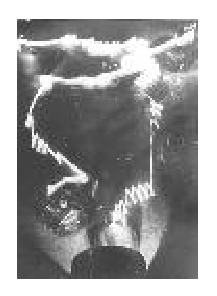
\includegraphics{notext_ps_logo}
\end{flushright}

  \vspace{3cm}	
  \centerline{ \Huge{Stage}}
  \vspace{0.5cm}
  \centerline{\Large{Version \VERSION\ User Manual}}
  \vspace{2cm}
  \centerline{\large   
	\begin{tabular}{l}
	  {\Large Richard T. Vaughan}\\Information Sciences Laboratory\\HRL Laboratories LLC\\Malibu, USA\\
  	\end{tabular} \\ 
	\begin{tabular}{r}
	  {\Large Andrew Howard}\\USC Robotics Labs\\University of Southern California\\Los Angeles, USA\\
	\end{tabular}
	}
  \vspace{1cm}

  \centerline{This document may not contain the most current documentation on}
  \centerline{Stage.  For the latest documentation, consult the Player/Stage homepage:}
  \centerline{{\tt http://playerstage.sourceforge.net}}

  \vspace{4cm}

 \centerline{\today}

\tableofcontents
%\newpage

%\listoffigures
%\newpage
%\listoftables
%\newpage

% reset page number to start with 1
\setcounter{page}{0}
\pagenumbering{arabic}


\chapter{Introduction}

  \section{What is Stage?}

    Stage simulates mobile robots and sensors in a two-dimensional
    bitmapped environment containing a variety of objects. Robots are
    controlled through Player. Player provides a powerful, flexible
    interface to the robots; Stage provides virtual devices for
    Player.  Various sensors and actuators are provided, including
    sonar, scanning laser rangefinders, vision (color blob detection),
    odometry, and both differential and omni-drive platforms.

	Stage is designed to support research into multi-agent
    intelligent autonomous systems.  Stage originated at the USC
    Robotics Research Labs to . One of the authors (

  \section{How to get Stage}

    The primary source for all things Player and Stage is:
      \begin{verbatim}
      http://playerstage.sourceforge.net
      \end{verbatim}	
   Official releases are available as source tarballs at:
      \begin{verbatim}
      http://playerstage.sourceforge.net
      \end{verbatim}
   The current development source is available by anonymous CVS from:
      \begin{verbatim}
      http://playerstage.sourceforge.net
      \end{verbatim}
The current release is Stage-\VERSION.

  \section{What's in the Package?}

    In the release tarball you will find:
      \begin{itemize}    
      \item stage    - the simulation engine.
      %\item manager  - a program for synchronizing several Stages distributed across
      %      multiple hosts. Experimental.
      %\item truthlog - a utility for logging the positions of all Stage's objects
      %	    (currently broken).
      \item Some example environments and setup files.
      \end{itemize}

  \section{Requirements}

    Stage was developed and tested under Linux kernel 2.4.2,
    glibc-2.2.2.  Written in reasonable ANSII/POSIX so should compile
    elsewhere. No promises, but people have found it to work on a
    variety of set-ups.

    Requires: Player [http://robotics.usc.edu/player/]
              TCP/IP, POSIX threads.
	Optional (but highly recommended): X11R6, GTK++.
  
  \section{Related Packages}

    A number of Player/Stage related packages can be found on the 
    Player website:
      \begin{verbatim}
      http://robotics.usc.edu/player
      \end{verbatim}
    Here you will find:
      \begin{itemize}
      \item Player : a networked robot device server.
      \item Stage : a multi-robot simulator.
      \item PlayerTools : a set of useful tools for interacting with
            Player/Stage.
      \item Sample clients for Player in C, Java and Python.
      \end{itemize}

  \section{Ownership}

    \noindent Stage is released under the GNU Public License.

    \noindent Stage programs, images, examples, source code and documentation are
    copyright (c) University of Southern California 1998-2001.

    \noindent Stage was created by:
      \begin{itemize}
      \item[] Richard Vaughan [rtv@sourceforge.net]
      \item[] Andrew Howard [inspectorg@sourceforge.net]
      \item[] Brian Gerkey [gerkey@sourceforge.net]
      \item[] Kasper Stoy [kaspers@robotics.usc.edu]
      \item[] Boyoon Jung [boyoon@robotics.usc.edu]
      \item[] Jakob Fredslund [jakobf@robotics.usc.edu]
      \end{itemize}

  \section{Bugs}
  
    This is research software, fresh off the presses.  As such, it is
    bound to contain bugs, despite our diligent testing.  If you
    manage to break something, or if some aspect of Stage's behavior
    seems wrong or non-intuitive, let us know.  Email should be sent
    to Richard Vaughan {\tt vaughan@hrl.com} or Andrew Howard {\tt
    ahoward@usc.edu}.  Include as much information as possible,
    including the Stage version, OS type and version, and any output
    messages.  A detailed description of what happened will enable us
    (hopefully) to repeat and analyze the problem.  Of course, there
    is NO WARRANTY on this software, and we are not paid to maintain
    it, so there is no guarantee that we will fix your problem.  But
    we will try :).

  \section{Names}
    
    From {\sl As You Like It} Act II, Scene 7:
    \begin{quote}
    ``All the world's a stage, \\
    And all the men and women merely players: \\
    They have their exits and their entrances; \\
    And one man in his time plays many parts,''\\
    \end{quote}

    From {\sl Macbeth} Act V, Scene 5:
    \begin{quote}
    ``Life's but a walking shadow, a poor player \\
    That struts and frets his hour upon the stage \\
    And then is heard no more: it is a tale \\
    Told by an idiot, full of sound and fury, \\
    Signifying nothing.''\\
    \end{quote}

  \section{Acknowledgements}

    Stage's development is supported at the University of Southern
    California by DARPA's TMR and MARS programs, and by an NSF grant.
    Richard Vaughan now works for HRL Laboratories, Malibu, CA.


\chapter{Running Stage}

  \section{Building and Installing Stage}

    {\bf You must install Player {\sl before} installing Stage.} 
    See:
      \begin{verbatim}
      http://robotics.usc.edu/player
      \end{verbatim}
    Once you've downloaded, built and installed Player, download
    the Stage tarball and unpack it with:
      \begin{verbatim}
      tar xzvf Stage-<version>.tgz
      \end{verbatim}
    Now follow the instructions in the top-level README file.

  \section{Running Stage}

    Before running stage, first make sure the Player executable can be
    found in your path (Stage will automatically start one or more
    instances of Player, so it needs to know where to find the Player
    executable).
    For example, try:
      \begin{verbatim}
      which player
      \end{verbatim}
    and make sure it returns a valid Player executable path, such as
      \begin{verbatim}
      /usr/local/player/bin/player
      \end{verbatim}
    If not, set your PATH variable to include the Player binary directory. 
    For example, in BASH do:
      \begin{verbatim}  
      export PATH=$PATH:/usr/local/player/bin
      \end{verbatim}  
    You should also make sure that the external viewer program XS
    can be found in your path.
    For example, try:
      \begin{verbatim}
      which xs
      \end{verbatim}
    and make sure it returns a valid executable path, such as
      \begin{verbatim}
      /usr/local/stage/bin/xs
      \end{verbatim}
    If not, set your PATH variable to include the XS binary directory;
    in BASH:
      \begin{verbatim}  
      export PATH=$PATH:/usr/local/stage/bin
      \end{verbatim}  
    To run stage itself do: 
      \begin{verbatim} 
      stage [options] <filename.world> 
      \end{verbatim} 
    The `.world' file specifies what stage must simulate. The
    command-line options are described below. If all is well, Stage
    will start up, load the world file, and spawn an instance of XS
    and Player. Each step causes a message on standard output, so a
    sample invocation and start up would look like this:
      \begin{verbatim}
      cd /usr/local/stage/examples
      stage simple.world 
 
      ** Stage v1.0 ** [World simple.world][./simple.pnm]        
      ** XS v0.4 ** [Env 6602][Truth 6601]
      ** Player v1.0 **
      \end{verbatim}
    Stage also outputs a status line on stdout at every cycle.  At
    this point you should be able to interact with objects in the
    world through XS and access sensors and actuators through
    Player. 
    Try using the Player example client:
      \begin{verbatim}
      viewer.tk
      \end{verbatim}
    to check that you can control Stage robots and read from their
    sensors. 
    You can also try the player-viewer program that comes as part of the
    PlayerTools package (available from the Player website).

    %Should probably have a Help! It didnt work section. AH
    %If it didn't work, the first things to check are the
    %settings in Makefile.common and your Player build.
  
  \section{Running RTKStage}

    RTKStage is a version of Stage compiled with a built-in X11 GUI
    using Andrew Howard's RTK toolkit. The RTK source is provided in
    the distribution (stage/rtk). This GUI provides some powerful
    features not found in XS.  Once you have setr up your paths
    as described above, you can start RTKStage using:
      \begin{verbatim} 
      rtkstage [options] <filename.world> 
      \end{verbatim} 
    RTKStage uses the same world files and command line options,
    but provides an alternative interface to the simulation.
    See Chapter \ref{sec:rtkstage} for more information on using
    RTKStage.

  \section{The World File}

    The world file is a description of the world that Stage
    must simulate.  It describes robots, sensors, actuators,
    moveable and immovable objects.  The world file can also
    be used to control many aspects of the simulation engine,
    such as its speed and fidelity.  
    See Chapter \ref{sec:world} for a complete description of
    the world file format.  Sample world files can also be
    found in the examples directory.

  \section{Command Line Arguments}

    Stage takes the following command-line options. Where an option
    can also be set in the configuration file, the command line option
    takes precedence.

    \begin{xarg}{-l <logfile>}
    Enables logging of device positions into the named file. This is
    useful for gathering experimental results, etc. The log file has a
    header that records information about the run.
    \end{xarg}

    \begin{xarg}{-xs}
    Prevents Stage spawing an instance of the XS GUI. RTKStage has this
    option enabled by default.
    \end{xarg}

    \begin{xarg}{+xs}
    Spawn an instance of XS.
    \end{xarg}

    \begin{xarg}{-u <update period in seconds>}
    Stage will attempt to take this much real time (wall-clock time)
    to perform each update cycle. It does this by computing the cycle,
    then sleeping (or polling for input) for any remaining time. If
    the cycle's computation takes longer than the requested cycle
    time, Stage will run slower than requested. Default is 0.1
    seconds.
    \end{xarg}

    \begin{xarg}{-v <simulation time step in seconds>}
    Stage will simulate the passing of this much time per update
    cycle. Default is 0.1 seconds. By changing the ratio of real (-u)
    and simulated (-v) time, you can make Stage run faster than,
    slower than, or approximately at real-time.
    \end{xarg}

    \begin{xarg}{-fast}
    Runs Stage as fast as possible. Stage will not attempt to match
    real time. Useful for batch runs and in sync mode (see
    below). This is slightly more efficient than setting the desired
    update time to zero seconds (-u 0.0).
    \end{xarg}

    \begin{xarg}{-tp <port num>}
    Set the port number for the "truth server" used by external
    clients such as XS and truthlogger. Default is 6602.
    \end{xarg}

    \begin{xarg}{-ep <port num>}
    Set the port number for the "enviornment server" used by external
    clients such as XS. Default is 6601.
    \end{xarg}

    %\begin{xarg}{-s}
    %Enable synchronized mode. If this option is given, Stage will wait
    %between update cycles for an external sync message. The Stage Manager
    %(bin/manager) tool uses this mode to connect and sychronize several
    %copies of Stage distributed over multiple hosts. 
    %\end{xarg}

\chapter{The World File}

The world file is used to describe the particular set of robots,
sensors and objects to be simulated by Stage.  Stage reads the world
file on start-up and creates entities as indicated in the file.  Stage
may also write updated pose information into the world file when the
user selects the {\bf File:Save} menu option.

\section{Basic Syntax}

A simple world file might look like this:
\begin{quote}
\begin{verbatim}
# This world file creates two robots with lasers.

environment 
( 
  file "cave.pnm" 
  scale 0.03 
)

position 
( 
  name "robot1" port 6665 pose [1 1 0] 
  player ()
  laser ()
)

position 
( 
  name "robot2" port 6666 pose [2 1 0] 
  player ()
  laser ()
)
\end{verbatim}
\end{quote}
This example shows the basic syntactic features of the 
world file format: comments, entities and properties.
%
Comments are indicated by the \verb'#' symbol; they may be placed
anywhere in the file and continue to the end of the line.  For
example:
\begin{quote}
\begin{verbatim}
# This world file creates two robots with lasers.
\end{verbatim}
\end{quote}
%
Entities are indicated using \verb'type ( ... )' entries; each such
entry instantiates an entity of type \verb'type'.  For example:
\begin{quote}
\begin{verbatim}
position ( ... )
\end{verbatim}
\end{quote}
creates a single position device (a bare-bones mobile robot).  Entities may
be nested to indicate that one entity is a ``child'' of another; thus:
\begin{quote}
\begin{verbatim}
position ( player () laser() )
\end{verbatim}
\end{quote}
creates a single position device with a Player server and laser attached to
it.  Think of child entities as physically sitting on their parent.
%
Entities have properties, indicated using \verb'name value' pairs:
\begin{quote}
\begin{verbatim}
position ( name "robot1" port 6665 pose [1 1 0] ... )
\end{verbatim}
\end{quote}
This entry creates a position device named ``robot1'' attached to port
6665, with initial position $(1, 1)$ and orientation of $0$.  Property
values can be either numbers (\verb'6665'), strings (indicated by
double quotes \verb'"robot1"') or tuples (indicated by brackets
\verb'[1 1 0]').

The above example can be re-written in a more concise form as follows:
\begin{quote}
\begin{verbatim}
# This world file creates two robots with lasers.
# It uses the 'define' construct to define a new type of entity.

environment ( file "cave.pnm" scale 0.03 )

define myrobot position ( player() laser() )

myrobot ( name "robot1" port 6665 pose [1 1 0] )
myrobot ( name "robot2" port 6666 pose [2 1 0] )
\end{verbatim}
\end{quote}
This example illustrates the use of the \verb'define newentity oldentity (...)'
construct do define new entity types.  For example, the line:
\begin{quote}
\begin{verbatim}
define myrobot position ( player() laser() )
\end{verbatim}
\end{quote}
defines a new \verb'myrobot' entity type composed of the
primitive \verb'position', \verb'player' and \verb'laser' entities.
This entity may be instantiated using the standard syntax:
\begin{quote}
\begin{verbatim}
myrobot ( name "robot1" port 6665 pose [1 1 0] )
\end{verbatim}
\end{quote}
This entry creates a position device named \verb'robot1' that has
both \verb'player' and \verb'laser' devices attached.

See the {\tt examples} directory in the Stage distribution for more
world file examples.


\section{Entity Summary}

\noindent
\begin{tabularx}{\columnwidth}{lX}
\hline 
\verb'environment' & \\
\verb'box' & \\
\verb'puck' & \\
\verb'laserbeacon' & \\
\hline
\end{tabularx}

\noindent
\begin{tabularx}{\columnwidth}{lX}
\hline
\verb'broadcast' & \\
\verb'gps' & \\ 
\verb'gripper' & \\
\verb'laser' & \\
\verb'lbd' & \\
\verb'misc' & \\
\verb'player' & \\
\verb'position' & \\
\verb'ptz' & \\
\verb'sonar' & \\
\verb'truth' & \\
\verb'vision' & \\
\hline
\end{tabularx}


\chapter*{Acknowledgements}
Player/Stage development is funded by DARPA under the Mobile Autonomous Robot Software
\end{document}
